\documentclass[openany]{ctexart}
\usepackage{amsmath,amssymb,amsthm,bm}
\usepackage{xcolor}
\definecolor{Solarized-base03}{RGB}{0, 43, 54}
\definecolor{Solarized-base02}{RGB}{7, 54, 66}
\definecolor{Solarized-base01}{RGB}{88, 110, 117}
\definecolor{Solarized-base00}{RGB}{101, 123, 131}
\definecolor{Solarized-base0}{RGB}{131, 148, 150}
\definecolor{Solarized-base1}{RGB}{147, 161, 161}
\definecolor{Solarized-base2}{RGB}{238, 232, 213}
\definecolor{Solarized-base3}{RGB}{253, 246, 227}
\definecolor{Solarized-yellow}{RGB}{181, 137, 0}
\definecolor{Solarized-orange}{RGB}{203, 75, 22}
\definecolor{Solarized-red}{RGB}{220, 50, 47}
\definecolor{Solarized-magenta}{RGB}{211, 54, 130}
\definecolor{Solarized-violet}{RGB}{108, 113, 196}
\definecolor{Solarized-blue}{RGB}{38, 139, 210}
\definecolor{Solarized-cyan}{RGB}{42, 161, 152}
\definecolor{Solarized-green}{RGB}{133, 153, 0}
\color{Solarized-base01}
\pagecolor{Solarized-base3}

\newcommand{\yellow}[1]{\textcolor{Solarized-yellow}{#1}}
\newcommand{\red}[1]{\textcolor{Solarized-red}{#1}}
\newcommand{\violet}[1]{\textcolor{Solarized-violet}{#1}}

\usepackage{fullpage}

\usepackage[bookmarksnumbered,bookmarksopen,colorlinks=true,citecolor=Solarized-green,anchorcolor=Solarized-blue,linkcolor=Solarized-blue,CJKbookmarks=true]{hyperref}

\usepackage{graphicx,epsfig,subfigure}
\usepackage{tikz,pgfplots}
\usepackage{ifthen}
\usetikzlibrary{backgrounds,automata,shapes,snakes,arrows,arrows.meta,chains,positioning,calc}
\usepackage[all]{xy}

\def \firstcircle{(90:1) circle (1.5)}
\def \secondcircle{(210:1) circle (1.5)}
\def \thirdcircle{(330:1) circle (1.5)}

\usepackage{kbordermatrix}

%\usepackage[charter]{newtxmath} % http://texdoc.net/texmf-dist/doc/fonts/newtx/newtxdoc.pdf
\setmainfont[]{EBGaramond08-Regular}
\setCJKmainfont[BoldFont=FZHei-B01]{FZLongZhao-R-GB}
\xeCJKsetup{CJKmath=true}
\everymath{\color{Solarized-magenta}}

\def \zerov {\bm{0}}
\def \onev {\bm{1}}
\def \av {\bm{a}}
\def \bv {\bm{b}}
\def \cv {\bm{c}}
\def \dv {\bm{d}}
\def \ev {\bm{e}}
\def \fv {\bm{f}}
\def \gv {\bm{g}}
\def \hv {\bm{h}}
\def \iv {\bm{i}}
\def \kv {\bm{k}}
\def \ov {\bm{o}}
\def \pv {\bm{p}}
\def \qv {\bm{q}}
\def \rv {\bm{r}}
\def \tv {\bm{t}}
\def \uv {\bm{u}}
\def \vv {\bm{v}}
\def \wv {\bm{w}}
\def \xv {\bm{x}}
\def \yv {\bm{y}}
\def \zv {\bm{z}}

\def \Av {\mathbf{A}}
\def \Bv {\mathbf{B}}
\def \Cv {\mathbf{C}}
\def \Dv {\mathbf{D}}
\def \Fv {\mathbf{F}}
\def \Gv {\mathbf{G}}
\def \Hv {\mathbf{H}}
\def \Iv {\mathbf{I}}
\def \Kv {\mathbf{K}}
\def \Lv {\mathbf{L}}
\def \Mv {\mathbf{M}}
\def \Pv {\mathbf{P}}
\def \Qv {\mathbf{Q}}
\def \Sv {\mathbf{S}}
\def \Uv {\mathbf{U}}
\def \Vv {\mathbf{V}}
\def \Wv {\mathbf{W}}
\def \Xv {\mathbf{X}}
\def \Yv {\mathbf{Y}}
\def \Zv {\mathbf{Z}}

\def \alphav {\bm{\alpha}}
\def \betav {\bm{\beta}}
\def \gammav {\bm{\gamma}}
\def \lambdav {\bm{\lambda}}
\def \Lambdav {\bm{\Lambda}}
\def \thetav {\bm{\theta}}
\def \epsilonv {\bm{\epsilon}}
\def \xiv {\bm{\xi}}
\def \muv {\bm{\mu}}
\def \Sigmav {\bm{\Sigma}}
\def \Phiv {\bm{\Phi}}
\def \nuv {\bm{\nu}}

\def \Acal {\mathcal{A}}
\def \Bcal {\mathcal{B}}
\def \Ical {\mathcal{I}}
\def \Lcal {\mathcal{L}}
\def \Ncal {\mathcal{N}}
\def \Pcal {\mathcal{P}}

\def \Dbb {\mathbb{D}}
\def \Ebb {\mathbb{E}}
\def \Nbb {\mathbb{N}}
\def \Qbb {\mathbb{Q}}
\def \Rbb {\mathbb{R}}
\def \Sbb {\mathbb{S}}

\def \Ifrak {\mathfrak{I}}
\def \Lfrak {\mathfrak{L}}
\def \Pfrak {\mathfrak{P}}

\def \diag {\mathrm{diag}}
\def \sign {\mathrm{sign}}
\def \sp {\mathrm{span}}
\def \diff {\mathrm{d}}
\def \tr {\mathrm{tr}}
\def \KL {\mathrm{KL}}
\def \var {\mathrm{var}}
\def \cov {\mathrm{cov}}
\def \ow {\mathrm{o.w.}}
\def \tanh {\mathrm{Tanh}}

\def \st {\mbox{s.t.}}
\def \const {\mbox{const}}

\DeclareMathOperator*{\argmin}{argmin}
\DeclareMathOperator*{\argmax}{argmax}

\allowdisplaybreaks[4]

\begin{document}
\title{}
\author{}
\date{}
\maketitle

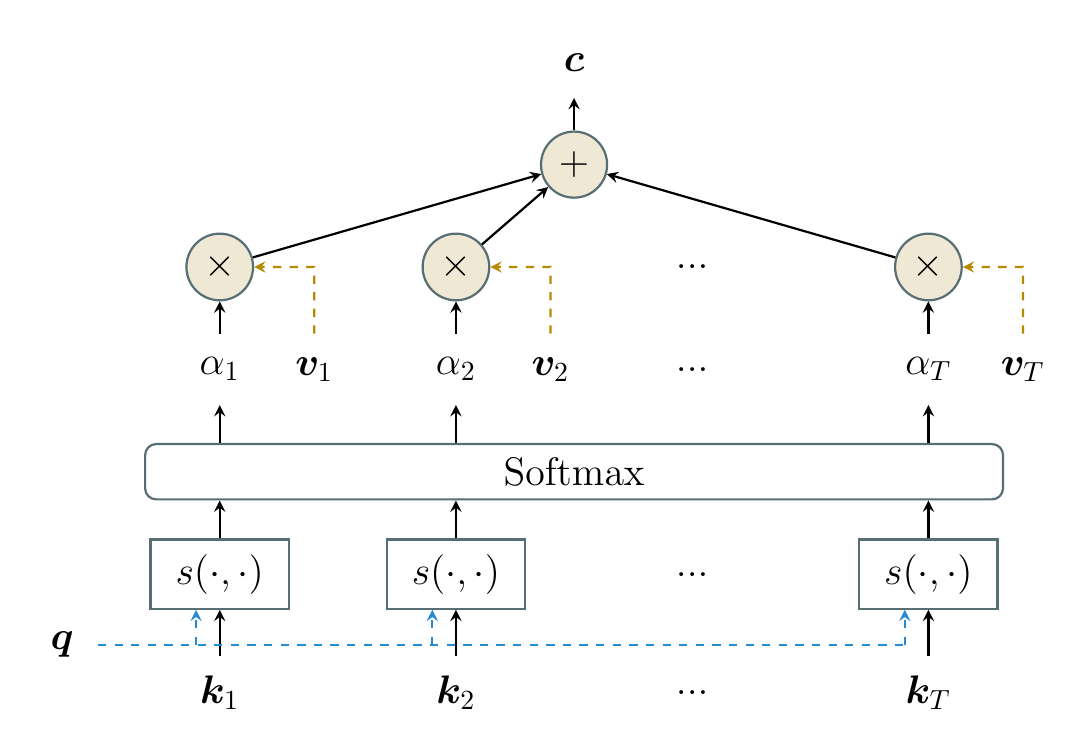
\begin{tikzpicture} [
    thick, >=stealth, scale=1, font=\Large, 
    box/.style = {rectangle,draw=Solarized-base01,minimum height=25,minimum width=50},
    plain/.style = {draw=none,minimum height=25,minimum width=25},
    roundbox/.style = {rounded corners,draw=Solarized-base01,minimum height=20,minimum width=310},
    op/.style = {circle,minimum width=20,draw=Solarized-base01,fill=Solarized-base2}
    ]

    \def \xarray{{-6,-3,0,3}}
    \def \yarray{{0, 1.5, 2.8, 4.1, 5.4, 6.7, 8.0}}

    \def \qxarray{{-6.3, -3.3, 2.7}}
    \pgfmathsetmacro{\qy}{0.6}

    \node (k1) [plain] at (\xarray[0], \yarray[0]) {$\kv_1$};
    \node (k2) [plain] at (\xarray[1], \yarray[0]) {$\kv_2$};
    \node (k3) [plain] at (\xarray[2], \yarray[0]) {...};
    \node (k4) [plain] at (\xarray[3], \yarray[0]) {$\kv_T$};

    \node (q) [plain] at (-8, \qy) {$\qv$};

    \node (s1) [box] at (\xarray[0], \yarray[1]) {$s(\cdot, \cdot)$};
    \node (s2) [box] at (\xarray[1], \yarray[1]) {$s(\cdot, \cdot)$};
    \node (s3) [plain] at (\xarray[2], \yarray[1]) {...};
    \node (s4) [box] at (\xarray[3], \yarray[1]) {$s(\cdot, \cdot)$};

    \node (s) [roundbox] at (-1.5, \yarray[2]) {Softmax};

    \node (a1) [plain] at (\xarray[0], \yarray[3]) {$\alpha_1$};
    \node (a2) [plain] at (\xarray[1], \yarray[3]) {$\alpha_2$};
    \node (a3) [plain] at (\xarray[2], \yarray[3]) {...};
    \node (a4) [plain] at (\xarray[3], \yarray[3]) {$\alpha_T$};

    \node (v1) [plain] at (\xarray[0]+1.2, \yarray[3]) {$\vv_1$};
    \node (v2) [plain] at (\xarray[1]+1.2, \yarray[3]) {$\vv_2$};
    \node (v4) [plain] at (\xarray[3]+1.2, \yarray[3]) {$\vv_T$};

    \node [op] (t1) at (\xarray[0], \yarray[4]) {$\times$};
    \node [op] (t2) at (\xarray[1], \yarray[4]) {$\times$};
    \node [plain] (t3) at (\xarray[2], \yarray[4]) {...};
    \node [op] (t4) at (\xarray[3], \yarray[4]) {$\times$};

    \node [op] (add) at (-1.5, \yarray[5]) {$+$};

    \node [plain] (c) at (-1.5, \yarray[6]) {$\cv$};

    \foreach \i in {1,2,4}
        {
            \draw[->] (k\i) -- (s\i);
            \draw[->] (s\i) -- (s.south -| s\i);
            \draw[<-] (a\i) -- (s.north -| a\i);
            \draw[->] (a\i) -- (t\i);
            \draw[->] (t\i) -- (add);
            \draw[->,Solarized-yellow,dashed] (v\i) -- ++(0, 1.3) -- (t\i);
        }

    \draw[->] (add) -- (c);

    \draw[Solarized-blue,dashed] (q) -- (\qxarray[2], \qy);

    \draw[Solarized-blue,dashed,->] (\qxarray[0], \qy) -- ($(s1.south east)!(\qxarray[0], \qy)!(s1.south)$);
    \draw[Solarized-blue,dashed,->] (\qxarray[1], \qy) -- ($(s2.south east)!(\qxarray[1], \qy)!(s2.south)$);
    \draw[Solarized-blue,dashed,->] (\qxarray[2], \qy) -- ($(s4.south east)!(\qxarray[2], \qy)!(s4.south)$);
    
\end{tikzpicture}




\end{document}

